\section{Theoretical Analysis}
\label{sec:analysis}

\subsection{Gain Stage}

\paragraph{} For the gain stage, the incremental stage provided the following results:

\begin{table}[h]
  \centering
  \begin{tabular}{|l|r|}
    \hline    
    {\bf Name} & {\bf Values} \\ \hline
    Input Z&489.187475 Ohm \\ \hline 
Output Z&726.398144 Ohm \\ \hline 
Gain&-212.967518 \\ \hline 
Gain(dB)&46.566267 dB \\ \hline 
 
  \end{tabular}
  \caption{Gain stage theoretical results}
  \label{tab:gain}
\end{table}

\paragraph{} From where we reach the conclusion that an output stage in necessary given the magnitude of the output impedance.

\subsection{Output Stage}

\paragraph{} The results of the output stage theoretical model are:

\begin{table}[h]
  \centering
  \begin{tabular}{|l|r|}
    \hline    
    {\bf Name} & {\bf Values} \\ \hline
    Input Z&9798.924013 Ohm \\ \hline 
Output Z&0.195570 Ohm \\ \hline 
Gain&0.995423 \\ \hline 
Gain(dB)&-0.039850 dB \\ \hline 
 
  \end{tabular}
  \caption{Output stage theoretical results}
  \label{tab:output}
\end{table}

\paragraph{} As we can see, the output impedance of this stage is much lower than the input. The output stage is also desirably low, specially when compared with the 8 Ohm of the speakers. At last, the total circuit gain results.

\begin{table}[h]
  \centering
  \begin{tabular}{|l|r|}
    \hline    
    {\bf Name} & {\bf Values} \\ \hline
    Input Z&489.187475 Ohm \\ \hline 
Output Z&3.130696 Ohm \\ \hline 
Gain&-197.362138 \\ \hline 
Gain(dB)&45.905277 dB \\ \hline 
 
  \end{tabular}
  \caption{Total circuit theoretical gain results}
  \label{tab:output}
\end{table}

\paragraph{} The frequency response of the circuit for the output voltage of the circuit, in terms of gain and phase difference, and the lower cut-off frequency are plotted here:

\begin{figure}[!h] \centering
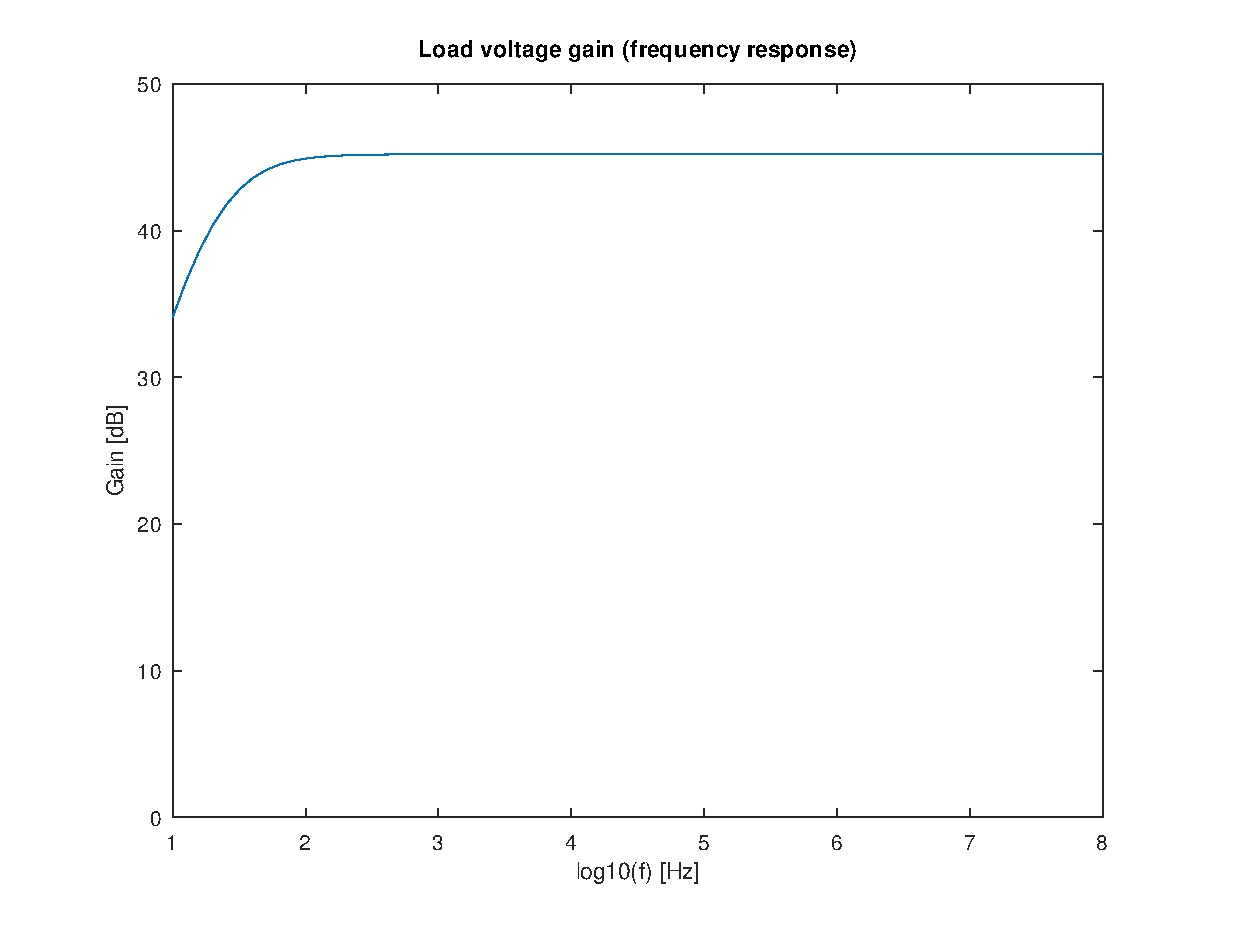
\includegraphics[width=0.6\linewidth]{Gain.eps}
\caption{Load output voltage gain (frequency response).}
\label{fig:gainfreq}
\end{figure}

\begin{figure}[!h] \centering
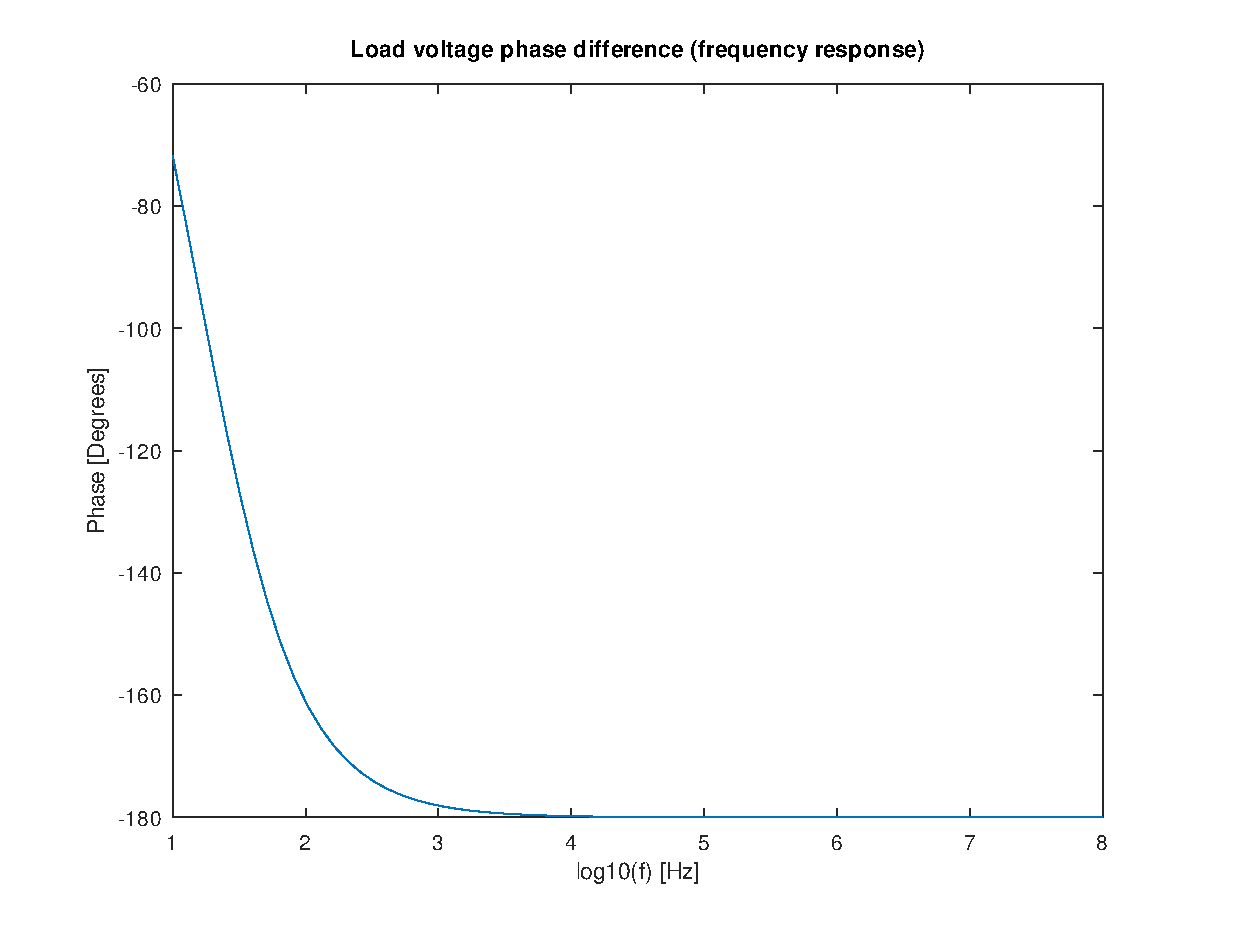
\includegraphics[width=0.6\linewidth]{Phase.eps}
\caption{Load output voltage phase difference (frequency response).}
\label{fig:phasefreq}
\end{figure}

\begin{table}[h]
  \centering
  \begin{tabular}{|l|r|}
    \hline    
    {\bf Name} & {\bf Values} \\ \hline
    Gain&182.000877 \\ \hline 
Gain(dB)&45.201470 dB \\ \hline 
Lower cut-off frequency&28.093870 Hz \\ \hline 
 
  \end{tabular}
  \caption{Gain for medium frequencies and lower cut-off frequency of the output voltage signal.}
  \label{tab:freq}
\end{table}

\clearpage
